\documentclass[a4paper,12pt]{article} % тип документа

% report, book

% Рисунки
\usepackage{graphicx}
\usepackage{wrapfig}
\usepackage{mathtext}
\usepackage[left=2cm,right=2cm,
    top=2cm,bottom=2cm,bindingoffset=0cm]{geometry}

\usepackage{hyperref}
\usepackage[rgb]{xcolor}
\hypersetup{				% Гиперссылки
    colorlinks=true,       	% false: ссылки в рамках
	urlcolor=blue          % на URL
}

%  Русский язык
\usepackage[T2A]{fontenc}			% кодировка
\usepackage[utf8]{inputenc}			% кодировка исходного текста
\usepackage[english,russian]{babel}	% локализация и переносы
\addto\captionsrussian{\def\refname{Список используемой литературы}}


% Математика
\usepackage{amsmath,amsfonts,amssymb,amsthm,mathtools} 
\usepackage{titlesec}
\titlelabel{\thetitle.\quad}

\usepackage{wasysym}
\title{3.3.4 Эффект Холла в полупроводниках}
\date{}

\begin{document}

\begin{center}
\textsf{\textbf{3.3.4A ЭФФЕКТ ХОЛЛА В ПОЛУПРОВОДНИКАХ}}
\end{center}

\textbf{Цель работы:} измерение подвижности и концентрации носителей заряда
в полупроводниках.

\textbf{В работе используются:} электромагнит с регулируемым источником питания; вольтметр; амперметр; миллиамперметр; миллитесламетр; источник питания, образцы легированного германия, программное обеспечение.

Перед выполнением работы необходимо ознакомиться с основами элементарной теории движения носителей заряда в металлах и полупроводниках (п. 4 введения к разделу).


Во внешнем магнитном поле $B$ на заряды действует сила Лоренца:
\begin{equation}
F = qE+qu\times B
\end{equation}

Эта сила вызывает движение носителей, направление которого в общем
случае не совпадает с $E$. Действительно, траектории частиц будут либо
искривляться, либо, если геометрия проводника этого не позволяет,
возникнет дополнительное электрическое поле, компенсирующее магнитную
составляющую силы Лоренца. Возникновение поперечного току
электрического поля в образце, помещённом во внешнее магнитное поле,
называют \textsf{эффектом Холла}.

\begin{figure}[h!]
\begin{center}
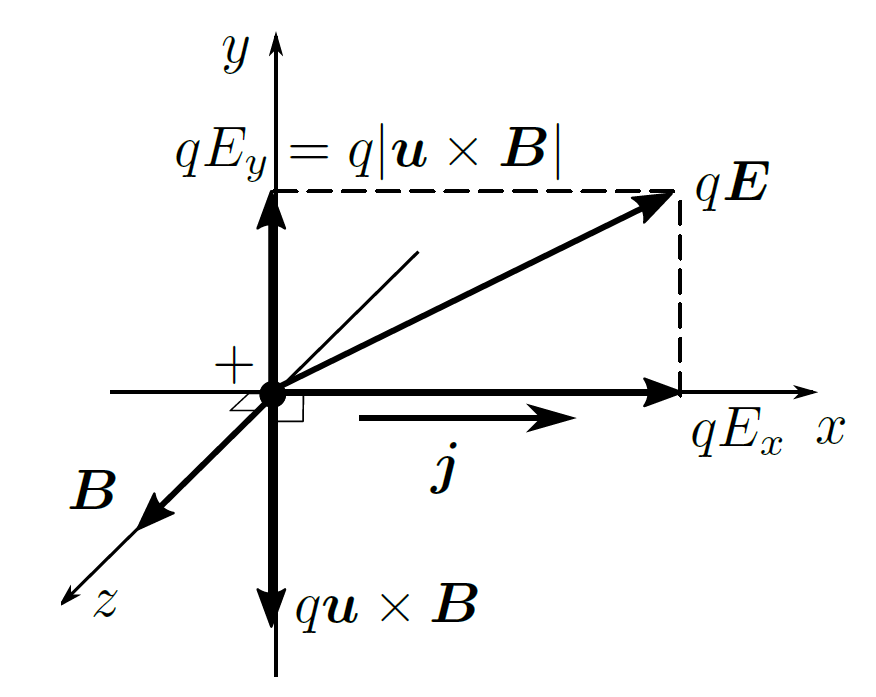
\includegraphics[width=0.46\textwidth]{Teor}
\caption{Силы, действующие на положительный носитель заряда в проводящей
среде при наличии магнитного поля} \label{силы}
\end{center}
\end{figure}

Пусть система содержит носители только одного типа (например,
электроны, как в большинстве металлов). Рассмотрим случай плоской геометрии: пусть ток течёт вдоль оси $x$, а магнитное поле направлено вдоль оси $x$ (см. рис. \ref{силы}). Магнитное поле действует на движущиеся заряды с силой $F_y=-qu_xB_z$ по оси $y$. Ток сможет
течь строго вдоль оси $x$, если заряды в среде перераспределятся таким
образом, чтобы полностью скомпенсировать магнитную силу, создав в
направлении $y$ электрическое поле:
\begin{equation}
\label{E_y}
E_y=u_xB_z=\dfrac{j_x}{nq}B_z
\end{equation}
называемое \textsf{холловским} (здесь $n$ — концентрация носителей). По оси
$x$ носители будут двигаться так, как если бы магнитного поля не было:
$j_x=\sigma_0 E_x (j_y = j_z = 0)$, где $\sigma_0 = qn\mu$ — удельная проводимость среды в отсутствие $B$.

Для исследования зависимости проводимости среды от магнитного
поля в данной работе используется \textsf{мостик Холла} (рис. \ref{мостик}).
\begin{figure}[h!]
\begin{center}
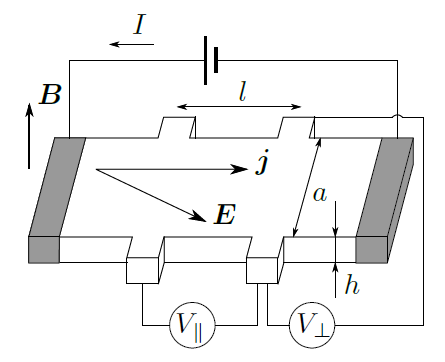
\includegraphics[width=0.46\textwidth]{Мостик}
\caption{Схема для исследования влияния магнитного поля на проводящие
свойства - мостик Холла} \label{мостик}
\end{center}
\end{figure}
В данной схеме ток вынуждают
течь по оси $x$ вдоль плоской пластинки (ширина пластинки $a$, толщина $h$,
длина $l$). Сила Лоренца, действующая со стороны перпендикулярного
пластинке магнитного поля, «прибивает» носители заряда к краям образца,
что создаёт холловское электрическое поле, компенсирующее эту
силу. Поперечное напряжение между краями пластинки (\textsf{холловское 
напряжение}) равно $U_\perp = E_ya$, где, согласно уравнению (\ref{E_y}):
\begin{equation}
E_y=u_xB_z=\dfrac{j_x}{nq}B
\end{equation}
Плотность тока, текущего через образец, равна $j_x=I/ah$, где $I$ — полный
ток, $ah$ — поперечное сечение. Таким образом, для холловского напряжения
имеем
\begin{equation}
U_\perp = \frac{B}{nqh}\cdot I=R_H\cdot \frac{B}{h}\cdot I,
\end{equation}
где константу
\begin{equation}
R_H = \frac{1}{nq}
\end{equation}
называют \textsf{постоянной Холла}. Знак постоянной Холла определяется
знаком заряда носителей.
Продольная напряжённость электрического поля равна
\begin{equation}
E_x=j_x/\sigma_0
\end{equation}
и падение напряжения $U_\parallel = E_x l$ вдоль пластинки определяется омическим
сопротивлением образца $R_0 = l/(\sigma_0 a h)$:
\begin{equation}
U_\parallel = IR_0
\end{equation}
 


Работа выполняется при помощи программного обеспечения, связь с приборами осуществляется через цифровой интерфейс RS-232 при помощи USB-портов.

В работе изучаются особенности проводимости полупроводников в
геометрии мостика Холла. Ток пропускается по плоской полупроводниковой пластинке, помещённой в перпендикулярное пластинке магнитное
поле. Измеряется разность потенциалов между краями пластинки в поперечном к току направлении. По измерениям определяется константа
Холла, тип проводимости (электронный или дырочный) и вычисляется концентрация основных носителей заряда на основе соотношения:
\begin{equation}
R_H = \frac{1}{nq},
\end{equation}
где $n$- концентрация основных носителей заряда, $R_H$ -постоянная Холла, $q$ - заряд носителя.

\textbf{Экспериментальная установка}
\begin{figure}[h!]
\begin{center}
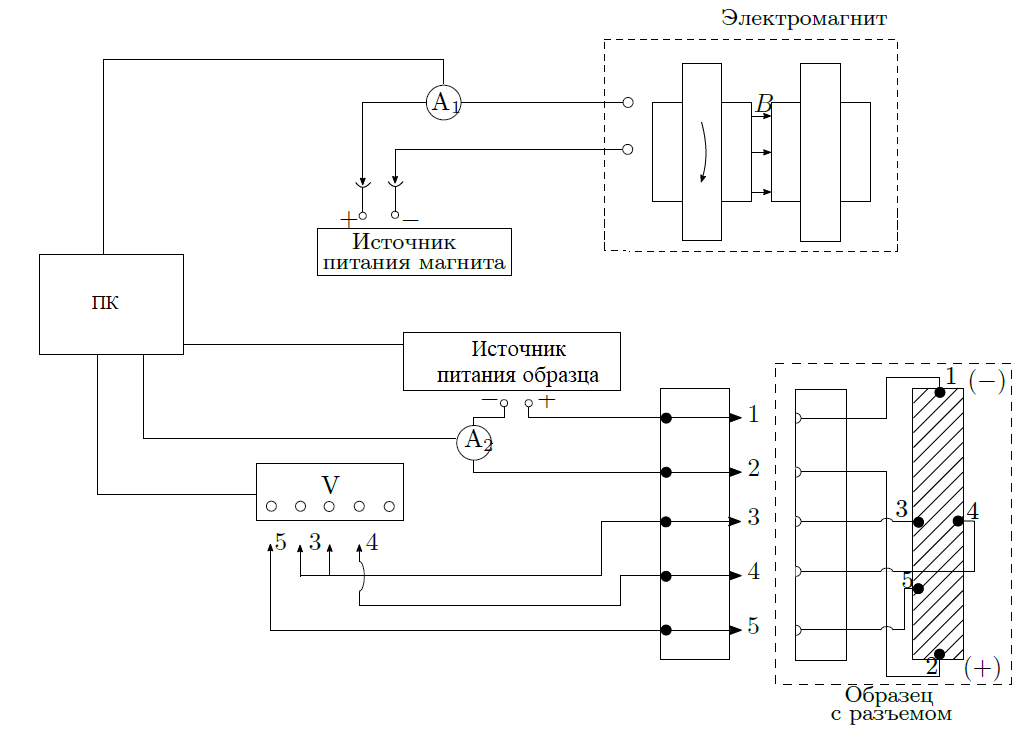
\includegraphics[width=0.76\textwidth]{Установка}
\caption{Схема установки для исследования эффекта Холла в полупроводниках} \label{установка}
\end{center}
\end{figure} 

Электрическая схема установки для измерения ЭДС Холла представлена на рис. \ref{установка}. В зазоре электромагнита (рис. \ref{установка}) создаётся постоянное
магнитное поле, величину которого можно менять с помощью регулятора источника питания электромагнита. Ток питания электромагнита измеряется внешним амперметром А1.

Градуировка электромагнита (связь тока с индукцией поля) проводится при помощи миллитесламетра на основе датчика Холла.

Прямоугольный образец из легированного германия, смонтированный в специальном держателе (рис. \ref{установка}), подключается к источнику питания образца. Вдоль длинной стороны образца течёт ток, величина которого регулируется на источнике питания образца и измеряется миллиамперметром А2.

В образце, помещённом в зазор электромагнита, между контактами 3
и 4 возникает разность потенциалов 34, которая измеряется с помощью
вольтметра V.

Контакты 3 и 4 вследствие неточности подпайки могут лежать не на
одной эквипотенциали. Тогда напряжение между ними связано не только с эффектом Холла, но и с омическим падением напряжения вдоль
пластинки. Исключить этот эффект можно, если при каждом значении тока через образец измерять напряжение между точками 3 и 4 в отсутствие магнитного поля. При фиксированном токе через образец это дополнительное к ЭДС Холла напряжение $U_0$ остаётся неизменным. От него следует (с учётом знака)
отсчитывать величину ЭДС Холла:
\begin{equation}
U_\perp = U_{34} - U_0
\end{equation}
При таком способе измерения нет необходимости проводить повторные
измерения с противоположным направлением магнитного поля.

По знаку $U_\perp$ можно определить характер проводимости — электронный или дырочный. Для этого необходимо знать направление тока в
образце и направление магнитного поля.

Измерив ток $I$ в образце и напряжение $U_{35}$ между контактами 3 и 5
в отсутствие магнитного поля, можно, зная параметры образца, рассчитать проводимость материала образца по формуле
\begin{equation}
\rho_0=\frac{U_{35}ah}{Il}
\end{equation}
где $l$ — расстояние между контактами 3 и 5, $a$ — ширина образца, $h$ —
его толщина.


\begin{center}
\textsf{\textbf{ЗАДАНИЕ}}
\end{center}
В работе предлагается исследовать зависимость ЭДС Холла от величины магнитного поля при различных значениях тока через образец для
определения константы Холла; определить знак носителей заряда и проводимость материала образца.


\begin{enumerate} 
	\item Работа будет состоять из 4 частей: градуировка электромагнита, измерение ЭДС Холла, определение знака носителей, измерение удельной проводимости.
  \item Соберите установку согласно схеме на рис. \ref{установка}, подключите к вольтметру контакты 3 и 4. Убедитесь, что источник питания электромагнита выключен, включите амперметры и вольтметр.
  \item Запустите программу <<Эффект Холла>>.
  \item Введите фамилие в поле <<Введите фамилию>>, нажмите клавишу ENTER.
  
\begin{center}
\textit{I. Градуировка электромагнита.}
\end{center}
  
  \item Для проведения градуировки электромагнита ознакомьтесь с устройством и принципом работы измерителя магнитной индукции ATE-8702. Техническое описание (ТО) расположено на установке.
  Включите измеритель индукции кнопкой <<POWER>>; через 2-3 секунды последовательным нажатием кнопки <<MODE>> установите режим измерения в постоянном поле  <<$a_1$>> (см. рис. 2 ТО).
  
  Снимите защитный колпачок с сенсорной головки датчика и коснитесь головкой поверхности магнита в зазоре.
  
  Для удержания показаний дисплея нажмите кнопку <<HOLD>>; повторное нажатие этой кнопки возвращает прибор в режим измерений.
  
  \item Установите ручки регулировки источника питания электромагнита в минимальное положение и нажмите на кнопку <<Градуировка электромагнита>>. Для начала эксперимента нажмите кнопку  <<Старт>>.
  
   Получите калибровочную кривую электромагнита: измерьте магнитную индукцию миллитесламетром, полученное значение введите в поле  <<Индукция>>, нажмите клавишу ENTER, измените ток питания электромагнита (на $5-7$ B). Повторите для 15-20 значений тока питания электромагнита.
   \item После окончания градуировки уберите миллитесламетр в коробку, выйдите в меню программы с помощью клавиши <<Меню>>.
   
\begin{center}
\textit{II. Определение ЭДС Холла.}
\end{center}   
   
  \item Вставьте образец в зазор электромагнита. Перейдите к определению ЭДС Холла кнопкой <<Определение ЭДС Холла>>.
  \item Введите $a$ в поле <<Введите a>>, нажмите клавишу ENTER. Установите ручки регулировки источника питания электромагнита в минимальное положение, нажмите кнопку <<Старт>>. Подождите, пока с приборов будет получено 15 значений.
\item Необходимо следить за ходом программы: получение данных может остановлено при слишком больших значения тока или после получения 15 точек.  
  
  \item Остановите процесс кнопкой  <<Стоп>>, измените ток на источнике питания электромагнита (на $8-12$ B). Запустите получение данных кнопкой  <<Новое напряжение>>. Повторите для 10-12 значений тока на источнике питания электромагнита.
     
\begin{center}
\textit{III. Определение знака носителей.}
\end{center}   

  \item После окончания основного эксперимента выйдете в основное меню программы кнопкой  <<Меню>>. Перейдите к определению знаку носителей заряда кнопкой <<Знак носителей>>.
  \item Определите знак носителей заряда в образце. Для этого необходимо
знать направление тока через образец, направление магнитного поля
и знак ЭДС Холла.

Направление тока в образце показано знаками  <<+>> и  <<->> на рис. \ref{установка}.
Направление тока в обмотках электромагнита при установке разъёма $K_1$ в положение 1 показано стрелкой на торце магнита. 

Измерьте разность потенциалов без магнитного поля (установите ручки регулировки источника питания электромагнита в минимальное положение, нажмите кнопку  <<Без поля>>). Подайте небольшое напряжение на электромагнит ($~10$ B), нажмите кнопку  <<С полем>>. Зафиксируйте результаты.

\begin{center}
\textit{IV. Измерение удельной проводимости.}
\end{center}  

\item Выключите источник питания электромагнита, перейдите в основное меню программы кнопкой  <<Меню>>. Перейдите к измерению удельной проводимости соответствующей кнопкой.
\item Удалите держатель с образцом из зазора электромагнита; подключите к клемма  <<U>> и  <<0>> вольтметра провода 3 и 5; введите параметры образца в соответствующие поля (после ввода обязательно нажать клавишу  <<ENTER>>). Введите $L$  в поле <<Введите L>> и $l$ в поле <<Введите l>>, нажмите кнопку  <<Старт>>.

\begin{center}
\textit{V. Обработка результатов.}
\end{center}  

\item Перейдите в основное меню программы. Для получения графиков и постоянных из эксперимента нажмите на кнопку  <<Обработка данных>>. 
\item Разберите установку, все полученные данные и графики хранятся в папке с вашей фамилией, сохраните их себе, например, на флешку.

\begin{center}
\textit{VI. Выводы.}
\end{center}  
\item Определите характер проводимости образца (дырочный или электронный) по направлению тока и по знаку постоянной Холла.

\item Сделайте вывод об адекватности полученных констант. При необходимости обработайте данные самостоятельно.
\end{enumerate}


\begin{center}
\textsf{\textbf{Контрольные вопросы.}}
\end{center}  

\begin{enumerate}

\item Какие вещества называют диэлектриками, проводниками, полупроводниками? Чем объясняется различие их электрических свойств? Как зависит
от температуры проводимость металлов и полупроводников?
\item Дайте определение константы Холла. Как зависит константа Холла от температуры у металлов и полупроводников?
\item Зависит ли результат измерения константы Холла от геометрии образца?
\item Зависит ли сопротивление образца от магнитного поля в условиях опыта?
\item Как устроен милливеберметр? Зависят ли его показания от сопротивления измерительной катушки? Каким должно быть это сопротивление по
сравнению с сопротивлением катушки прибора?
\item По результатам измерений оцените частоту столкновений, длину пробега
и коэффициент диффузии носителей тока в образце.
\item Получите выражение константы Холла для материалов с двумя типами носителей. Указание: воспользуйтесь условием равенства нулю поперечного
тока.
  
\end{enumerate}

\end{document}